%% ----------------------------------------------------------------------------
% BIWI SA/MA thesis template
%
% Created 09/29/2006 by Andreas Ess
% Extended 13/02/2009 by Jan Lesniak - jlesniak@vision.ee.ethz.ch
%% ----------------------------------------------------------------------------
\newpage
\chapter{Materials and Methods}
The objectives of the ``Materials and Methods'' section are the following:
\begin{itemize}
    \item \textit{What are tools and methods you used?} Introduce the environment, in which your work has taken place - this can be a software package, a device or a system description. Make sure sufficiently detailed descriptions of the algorithms and concepts (e.g. math) you used shall be placed here.
    \item \textit{What is your work?} Describe (perhaps in a separate chapter) the key component of your work, e.g. an algorithm or software framework you have developed.
\end{itemize}
\section{Latent Variable Models}
Before getting started it is important to define the terms used in the next sections, since they all stem from Bayesian
statistics. The Bayesian theorem can be written as
\begin{equation}
    p(z|x) = \frac{p(x|z)p(z)}{p(x)}
\end{equation}
where it is implicitly assumed that $p$ is a probability density function over two continuous random variables $x$ and $z$. The formula holds in general, but in generative modeling and machine learning it is usually assumed that the letter $z$ represents a random variable in a latent (unobserved) space from which -- after successful training -- new data can be generated by sampling. This requires that $p(z)$ is a simple distribution from which sampling is easy and that the trained model is capable of mapping values from the latent distribution to the true data distribution.

Using above described ordering, the four terms in this formula use distinct names:
\begin{description}
    \item[$p(x)$] is called the \textit{evidence} or the \textit{marginal likelihood}. It encompasses the actual observations of the data.
    \item[$p(z)$] is called the \textit{prior}, since it exposes information on $z$ before any conditioning.
    \item[$p(z|x)$] is called the \textit{posterior}. It describes the distribution over $z$ after (\textit{post}) having seen the evidence $x$.
    \item[$p(x|z)$] is called the \textit{likelihood}. It gives the literal likelihood of observing an example $x$ when choosing the latent space to be a specific $z$.
\end{description}

\section{Variational Autoencoders}
One of the most straightforward examples of a generative model, where the goal is to find such a latent space representation of the training sample distribution, is the Variational Autoencoder (VAE)~\autocite{kingma2022autoencoding}. The name of the VAE stems from the Autoencoder, a network that tries to recreate its output through a bottleneck and thereby learns a compressed representation of the data.~\autocite{https://doi.org/10.1002/aic.690370209} Autoencoders bear similarity to other dimension reduction methods like Principal Component Analysis (PCA) and therefore were first published under the name \textit{Nonlinear principal component analysis}. The \textit{variational} part in the VAE stems from the fact that it does not only learn to recreate input samples through dimensionality reduction, but is also optimized to represent the distribution over the training samples as a combination of a parameterized latent distribution $p_{\theta_z}(z)$ and a neural network mapping $p_{\theta_{NN}}(x|z)$ between the latent space and the sample space, termed decoder. The latent distribution is chosen such that sampling from it is easy (e.g. a multivariate Gaussian, with the parameters being vectors of means and variances). With sufficient dimensionality reduction the encoding should not overfit and the latent space should be a good approximation of the true data manifold. This enables the creation of data, by sampling the latent space and mapping it to the output.

Marginalizing $p_\theta(x)$ requires another approximation of the posterior $p(z|x)$ with a neural network, termed the encoder $p_{\theta_{NN_{in}}}(z|x)$.
\begin{equation}
    p_{\theta}(x) = \int p_{\theta_{NN}}(x|z) p_{\theta_z}(z) dz = \frac{p_{\theta_{NN_{out}}}(x|z) p_{\theta_z}(z)}{p_{\theta_{NN_{in}}}(z|x)}
\end{equation}
A schematic of a VAE, separated into these 3 factors -- encoder, latent distribution and decoder -- is shown in Fig.~\ref{fig:vae}.
\begin{figure}[h]
    \centering
    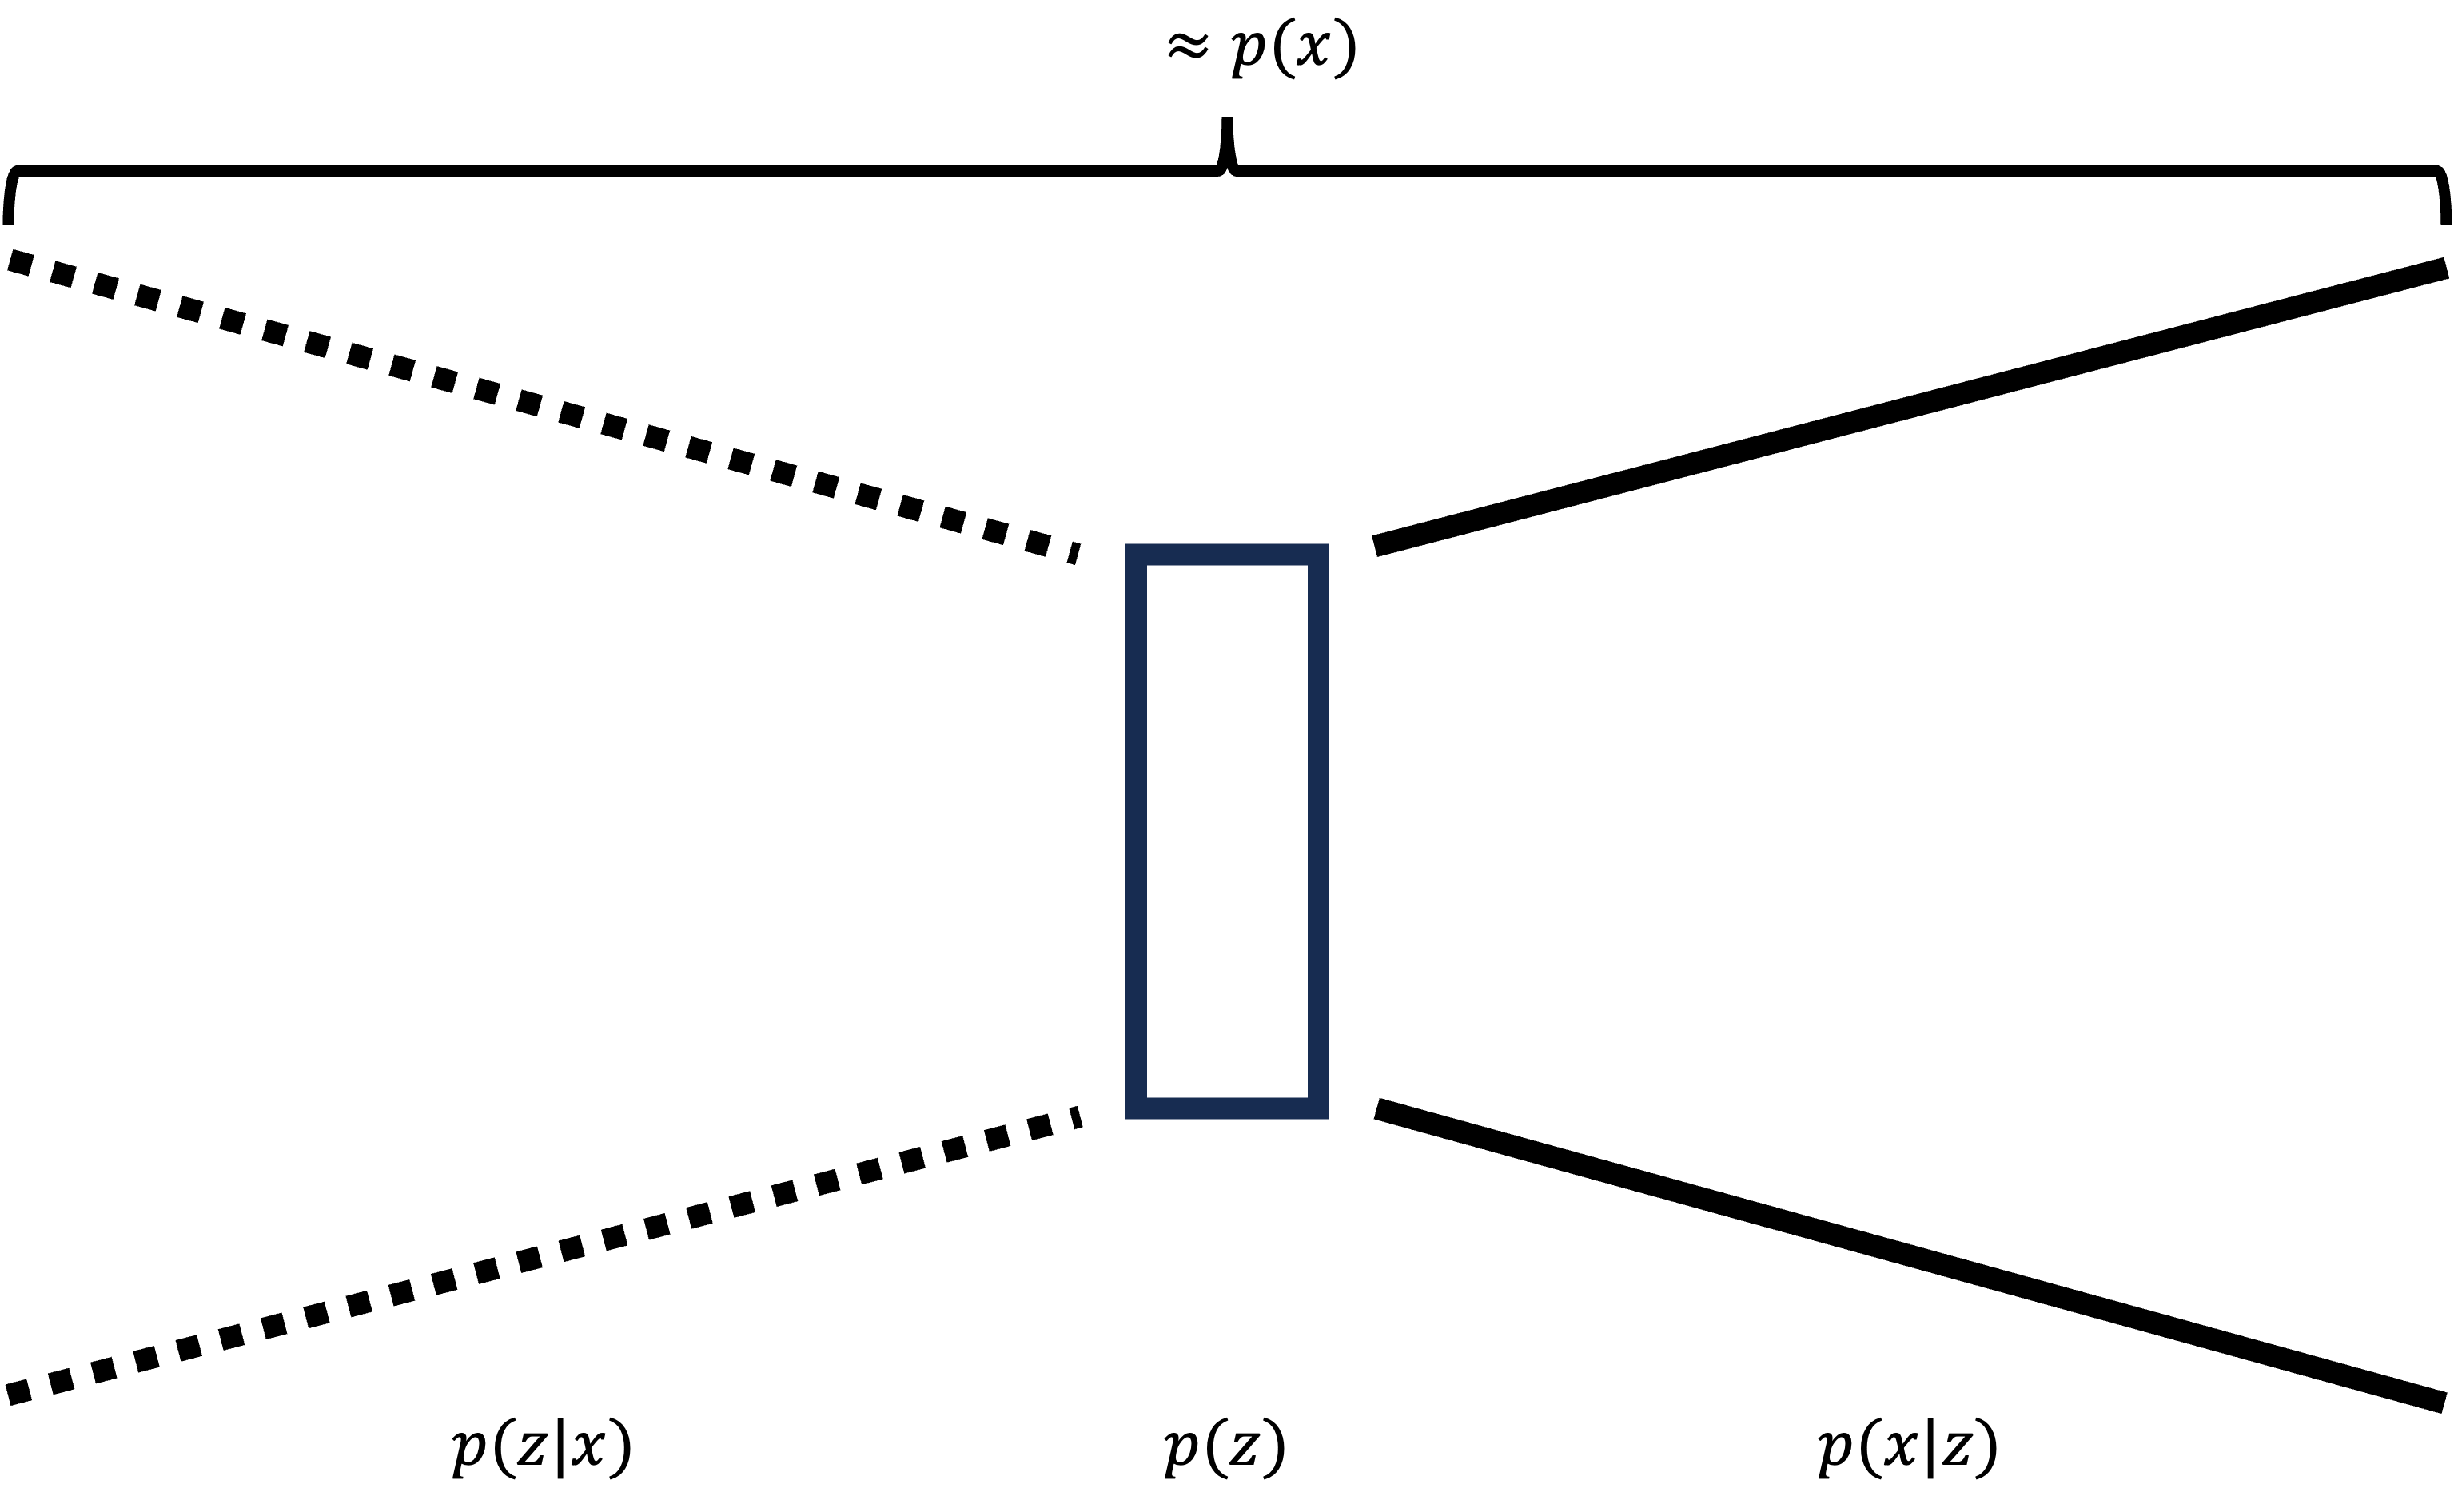
\includegraphics[width=.5\textwidth]{images/vae.png}
    \caption{VAE schematic: $p(x)$ is approximated through a latent variable model where posterior and likelihood are modeled with neural networks and the prior on the latent variable is modeled through a simple parameterized distribution (often Gaussian). The hope is, that after training, sampling from $p(z)$ and passing it through the neural network $p_{\theta_{NN}}(x|z)$, is the same as sampling from $p(x)$.}
    \label{fig:vae}
\end{figure}

\section{KL Divergence and Variational Lower Bound}
In VAEs, the encoder $p_{\theta}(z|x)$ needs to approximate the posterior $p(z|x)$, therefore a differentiable loss function is needed that compares two probability distributions. One such heavily used measure is the KL (Kullback-Leibler) divergence
\begin{equation}
    KL\left[p_{\theta}(z|x) || p(z|x)\right] = \int \log \frac{p_{\theta}(z|x)}{p(z|x)} p_{\theta}(z|x) dz
\end{equation}
which has the properties of being strictly non-negative and is only 0 if the two distributions are equal.

At the same time, the output of the VAE should fit the true data distribution well, e.g. should maximize the log-likelihood of the evidence $p_{\theta}(x|z)$. This term is mainly responsible for the reconstruction of truthful samples from the latent space. Combining the two terms and inverting the signs (for minimization rather than maximization) gives a loss function known as ELBO (evidence lower bound) or VLB (variational lower bound).
\begin{equation}
    \label{eq:elbo}
    \mathcal{L}_{VLB} = - \log p_{\theta}(x|z) + KL\left[p_{\theta}(z|x) || p(z|x)\right]
\end{equation}

\section{Diffusion Denoising Probabilistic Models}
Diffusion Denoising Probabilistic Models (DDPMs or Diffusion Models) are a generative model that learn the distribution of images in a training set. During training, sample images are gradually destroyed by adding noise over many iterations and a neural network is trained, such that these steps can be inverted.

As the name suggests, image content is diffused in timesteps, therefore we use the random variable $\bm{x}_0$ to represent our original training images, $\bm{x}_t$ for (partially noisy) images at an intermediate timestep and $\bm{x}_T$ for images at the end of the process where all information has been destroyed and the distribution $q(\bm{x}_T)$ largely follows an isotropic Gaussian distribution.

The goal is to train a network that creates a less noisy image $\bm{x}_{t-1}$ from $\bm{x}_t$. If this is achieved we should be able to sample some new $\bm{x}_T$ and generate new samples from the training distribution $q(\bm{x}_0)$ by passing this noisy image many times through the network until the noise is fully removed.

\subsection{Forward Diffusion Process}
\subsubsection{Mathematical Description}
In order to derive a training objective it is important to understand the workings of the \textit{forward diffusion process}. During this process, i.i.d (independent and identically distributed) Gaussian noise is applied to the image over many discrete timesteps. A \textit{variance schedule} defines the means and variances ($\sqrt{1-\beta}$ and $\beta$) of the added noise at every timestep.~\autocite{ho2020denoising} The whole process can be expressed as a Markov chain (depicted in Fig.~\ref{fig:forward_diffusion}), with the factorization
\begin{equation}
    \label{eq:forwardprocess}
    q(\bm{x}_T|\bm{x}_0) = q(\bm{x}_0) \prod_{t=1}^{T} q(\bm{x}_{t}|\bm{x}_{t-1})
\end{equation}
where the transition distributions $q(\bm{x}_t|\bm{x}_{t-1}) = \mathcal{N}(\sqrt{1-\beta_t} \bm{x}_{t-1}, \beta_t I)$. An example of iterative destruction of an image by this process is shown in Fig.~\ref{fig:forward_naoshima}.

\begin{figure}[h]
    \centering
    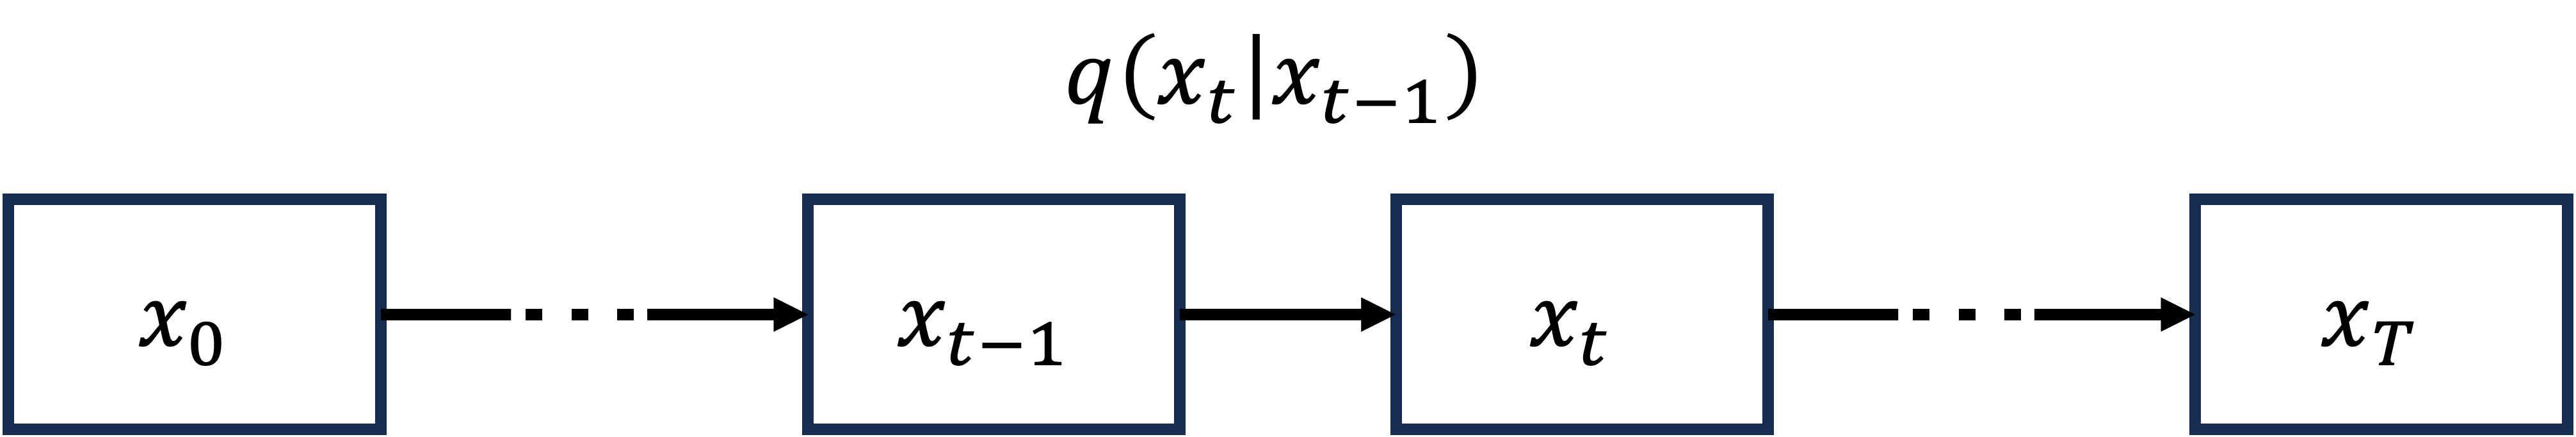
\includegraphics[width=.5\textwidth]{images/forward_diffusion.png}
    \caption{Forward Diffusion Process: An image is iteratively destroyed by adding normally distributed noise,
        according to a schedule. This represents a Markov process with the transition probability $q(\bm{x}_t|\bm{x}_{t-1})$.}
    \label{fig:forward_diffusion}
\end{figure}

\begin{figure}[h]
    \centering
    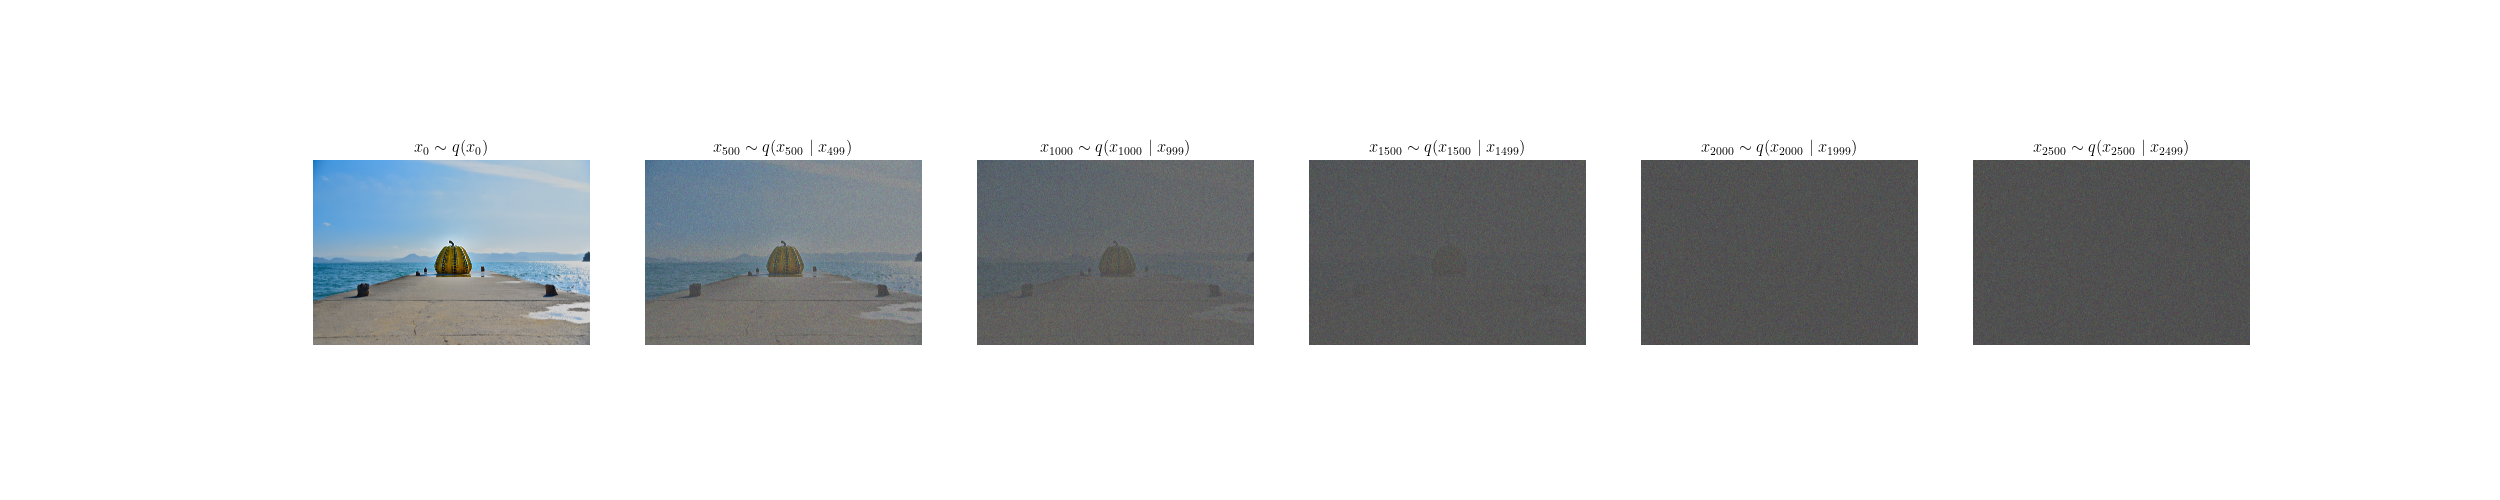
\includegraphics[width=\textwidth]{images/forward_naoshima.png}
    \caption{Example of Iterative Image Destruction through Forward Diffusion Process:
        The indices give the time step in the iterative destruction process, where $\beta$ was created according to a linear noise variance schedule (5000 steps from in the 0.001 to 0.02 range and picture resolution of 4016 by 6016 pixels).}
    \label{fig:forward_naoshima}
\end{figure}

Gladly it is not necessary to sample noise again and again in order to arrive at $\bm{x}_t$, since Ho et al. derived a closed-form solution to the sampling procedure.~\autocite{ho2020denoising} For this, the variance schedule is first reparameterized as $1-\beta = \alpha$
\begin{equation}
    q(\bm{x}_t | \bm{x}_{t-1}) = \mathcal{N}(\sqrt{\alpha_t} \bm{x}_{t-1}, (1-\alpha_t) \bm{I})
    \label{eq:forward_alpha}
\end{equation}
and the closed-form solution for $q(\bm{x}_t|\bm{x}_0)$ is derived by introducing the cumulative product $\bar{\alpha_t} = \prod_{s=1}^{t}\alpha_s$ as
\begin{equation}
    q(\bm{x}_t|\bm{x}_0) = \mathcal{N}(\sqrt{\bar{\alpha_t}}\bm{x}_0, (1-\bar{\alpha_t})\bm{I})
    \label{eq:forward_alphadash}
\end{equation}
A choice of $\bar{\alpha_t} \in [0,1]$ in above parameterizaiton ensures that the variance does not explode in the process, but that the SNR (signal-to-noise-ratio) still goes to 0 by gradually attenuating the means, corresponding to the original image. Thanks to the reparameterization with $\bar{\alpha_t}$, the forward process is also not restricted anymore to discrete timesteps, but a continuous schedule can be used.~\autocite{kingma2023variational,song2021scorebased}

The derivation that leads from Eq.~\ref{eq:forward_alpha} to Eq.~\ref{eq:forward_alphadash} is left to appendix~\ref{app:forward}.

\subsubsection{Influence of Scheduling Functions}
The process of information destruction is dependent on the chosen variance schedule, the number of steps and the image size. Beyond the most simple case -- a constant variance over time -- Ho et al. opted for the second most simple option, a linear schedule, where the variance $\beta_t$ grows linearly in $t$.~\autocite{ho2020denoising} Nichol et al. later found that a cosine-based schedule gives better results on lower resolution images, since it does not destruct information quite as quickly, making it more informative in the last few timesteps. They also mention that their cosine schedule is purely based on intuition and they similar functions to perform equally well.~\autocite{nichol2021improved}  Own experiments exploring above mentioned parameters are explained in~\ref{sec:forward_diff_experiments} and plots of the two different variance schedules are visible in Fig.~\ref{fig:alphadash}.

\subsection{Reverse Diffusion Process}
DDPMs can be viewed as latent space models in a similar way that Generative Adversarial Nets or Variational Autoencoders can.~\autocite{goodfellow2014generative,kingma2022autoencoding}

In DDPMs the reverse process is again a Markov chain and can therefore again be factorized as
\begin{equation}
    \label{eq:reverseprocess}
    q(\bm{x}_0|\bm{x}_T) = q(\bm{x}_T) \prod_{t=T}^{1} q(\bm{x}_{t-1}|\bm{x}_{t})
\end{equation}
which means that our network does not learn to approximate the full inversion, but rather just the transition probabilities $q(\bm{x}_{t-1}|\bm{x}_{t})$ in the chain, which are transitions between several intermediate latent distributions. Sohl-Dickstein et al. further showed that the reverse transitions are also Gaussian in the limit of $t \rightarrow 0$, e.g. as long as the diffusion steps are small enough. We therefore approximate
\begin{equation}
    \label{eq:reverseapprox}
    q(\bm{x}_{t-1} | \bm{x}_t) \approx p_{\theta}(\bm{x}_{t-1} | \bm{x}_t) = \mathcal{N}(\bm{\mu}_{\theta}(\bm{x}_t, t),\bm{\Sigma}_{\theta}(\bm{x}_t, t)).
\end{equation}

\subsection{Loss Functions}
The combination of forward $q(\bm{x}_T|\bm{x}_0)$ and reverse process $q(\bm{x}_0|\bm{x}_T)$ can be viewed as a chain of many VAEs and we can again formulate a variational lower bound objective (Eq.~\ref{eq:elbo}) that maximizes log-likelihood of the output and matches transition probabilities.~\autocite{nichol2021improved}
\begin{align}
    \mathcal{L}_0       & = - \log p_{\theta}(x_0|x_1)                                    \\
    \mathcal{L}_{1:T-1} & = KL\left[q(x_{t-1}|x_t, x_0) || p_{\theta}(x_{t-1}|x_t)\right] \\
    \mathcal{L}_T       & = KL\left[q(x_T|x_0) || p(x_T)\right]
\end{align}
The exact posterior $q(x_{t-1}|x_t, x_0)$ is tractable for specific samples of the training distribution, therefore $\mathcal{L}_{1:T-1}$ could be calculated, since KL divergence has a closed form solution for two Gaussian distributions. $\mathcal{L}_T$ is independent of $\theta$ and therefore not used for optimization. It should anyway be very close to zero if the parameterization of the forward process is correct and forward diffused samples get close to $\mathcal{N}(0,\bm{I})$. The first term is only used for performance evaluation in terms of log-likelihood, but not in optimization.

Another simplification is usually taken and $p_{\theta}(\bm{x}_{t-1} | \bm{x}_t)$ only approximates the means $\bm{\mu}_{\theta}$ and not the variances. For small enough timesteps, the means determine the transitional distributions much stronger than the variances. The network is furhter usually trained to not predict the means directly, but the noise and the means are then determined through a reparameterization.~\autocite{ho2020denoising,nichol2021improved}

\section{Image Guided Diffusion}
Both, Choi et al. and Lugmayr et al. make use of unconditional DDPMs for image-guided diffusion for the tasks of image translation in the former and in-painting in the latter.~\autocite{choi2021ilvr,lugmayr2022repaint} Similarly, classifier guidance or CLIP-guidance can be used on unconditional and conditional DDPMs to produce samples of a specific class or matching a prompt in the unconditional case or to further trade off sample variability for sample fidelity.~\autocite{dhariwal2021diffusion} We show here that both approaches can be interpreted as special cases of MAP (maximum a posteriori) estimation and that they can be generalized to other means of guidance during the reverse process.
\subsection{MAP Estimation for Inverse Problems}
MAP estimation is a statistical concept that is often used for optimizing the parameters $\theta$ of a parameterized distribution to observed data $z\sim p(z)$ following Bayes rule
\begin{equation}
    \hat{\theta}_{MAP} = \argmax_{\theta} p(\theta | z) = \argmax_{\theta}\frac{p(z|\theta)p(\theta)}{p(z)}
\end{equation}
or for inverse problems
\begin{equation}
    \hat{x}_{MAP} = \argmax_x p(x|s) = \argmax_x \frac{p(s|x)p(x)}{p(s)}
\end{equation}
where $s \sim p(s)$ is the evidence that is provided by the measured signal, $p(x)$ is a prior on the desired reconstruction and the likelihood term $p(s|x)$ enforces a data consistency between the measured signal and the true distribution, usually a forward model of the data-corrupting process. Since maximizing $p(x|s)$ is the same as maximizing $\log(x|s)$ and $p(s)$ is independent of $\theta$, we can separate the product into a sum.
\begin{align}
    \hat{x}_{MAP} = \argmax_x log p(x|s) & = \argmax_x \log{\frac{p(s|x)p(x)}{p(s)}} \\
                                         & = \argmax_x \log p(s|x)p(x)               \\
                                         & = \argmax_x \log f(x, s)
\end{align}
Such problems are usually optimized using iterative optimization schemes such as gradient ascent $x_{t+1} = x_{t} + \lambda \nabla_{x} f(x, s)$, with $\lambda$ being the step length. It is usually helpful to separate the data consistency term (likelihood) and regularizer (prior) into individual terms for joint optimization with their respective gradients and weights.
\begin{align}
    \label{eq:mapestimation}
    x_{i+1} = x_{i} + \lambda_1 \nabla_{x_i} \log p(s|x_i) + \lambda_2 \nabla_{x_i} \log p(x_i)
\end{align}

\subsection{DDPMs as Priors}
DDPMs approximate a data distribution over training images $p(x)$ and according to Song et al., they do so by learning to approximate gradients of the distribution and taking a gradient ascent step with every iteration of the reverse diffusion process.~\autocite{song2020generative} With this interpretation the DDPM has the exact same form as Eq.~\ref{eq:mapestimation} without the data consistency term $p(s|x)$.
\begin{equation}
    \label{eq:ddpmiteration}
    x_{t-1} = x_{t} + \nabla_{x_t} \log p(x_t)
\end{equation}

\subsection{Classifier Guidance}
Classifier guidance as termed by Nichol et al. introduces a data consistency term $p(s|x_t)$ in the form of a classifier trained on noisy images, where $s$ is the random variable expressing if an image belongs to a certain class.~\autocite{dhariwal2021diffusion,sohldickstein2015deep} Conditioning on a classifier is sucessfully used by taking gradient ascent steps not only in the direction that maximizes the prior $p(x)$ in a DDPM $\nabla_{x_t} \log p(x_t)$, but also the direction of this conditioning term $\nabla_{x_t} \log p(s|x_t)$. In total, this is equal to Eq.~\ref{eq:mapestimation}
\begin{equation}
    x_{t+1} = \underbrace{x_{t} + \nabla_{x_t} \log p(x_t)}_{x'_{t+1}} + \lambda \nabla_{x_t} \log p(s|x_t)
\end{equation}
with $x'_{t+1}$ being the prediction of the reverse diffusion steps before any conditioning and $\lambda$ an arbitrary factor determining the strength of the guidance.

\subsection{Gradients and Closed-Forms of Data Consistency Terms}
Starting from Eq.~\ref{eq:ddpmiteration}, the data consistency term can be reintroduced into the DDPM model.

Choi et al. guide the diffusion process by trying to match the low frequency content of a target image to the low frequency content of the prediction $\argmin_x \phi(s) - phi(x)$. They do this by using a very simple linear data consistency function, corresponding to a difference between linear low-pass filtered representations, which they call ILVR (iterative latent variable refinement)
\begin{align}
    \label{eq:ilvr}
    x_{t-1} & = \phi(s_{t}) + (I - \phi) (x_{t})  \\
    x_{t-1} & = x_{t} + \phi(s_{t}) - \phi(x_{t}) \\
    x_{t-1} & = x_{t} + \phi(s_{t} -x_{t})
\end{align}
where $\phi$ is a linear filter operation and $s_t$ is obtained by using the forward process on the target image.~\autocite{choi2021ilvr}

Similarly, Lugmayr et al. use a conditioning on known parts of the image for the inpainting operation, which effectively boils down to applying a linear mask that zeroes out known parts in the prediction and replaces them with outputs from the forward process.
\begin{align}
    \label{eq:repaint}
    % Mx_t (0 at unknown, 1 at known) removes known parts from x_t and leaves unknown
    % Ms_t (0 at unknown, 1 at known) leaves prediction in unknown region and replaces known region
    x_{t-1} & = x_t - \mathcal{M}(x_t) + \mathcal{M}(s_t) \\
    x_{t-1} & = x_t + \mathcal{M}(s_t - x_t)
\end{align}
As is easily seen, Eq.~\ref{eq:ilvr} and Eq.~\ref{eq:repaint} take the same form and can be interpretated as simultaneously taking gradient ascent steps for optimizing $\argmax_x \log p(x)$ and $\argmax_x \log p(s|x)$.

Assuming distribution over latent predictions and targets at diffusion timestep $t$, $p(s|t)$ and $p(x|t)$, and $\mathcal{L}$ corresponding to an arbitrary linear operation
\begin{align}
    \mathcal{L}(p(s|t) - p(x|t))                                                       & = \nabla_{x_t} \log p(s_t|x_t)         \\
    \int \mathcal{L}(p(s|t) - p(x|t)) dt                                               & = \int \nabla_{x_t} \log p(s_t|x_t) dt \\
    \int \mathcal{L}(p(s|t))dt - \int \mathcal{L}(p(x|t))dt                            & = \log p(s|x)                          \\
    \mathcal{L} \left(\int p(s|t)dt \right) - \mathcal{L} \left( \int p(x|t)dt \right) & = \log p(s|x)                          \\
    \mathcal{L}(p(s)) - \mathcal{L}(p(x))                                              & = \log p(s|x)
\end{align}
where the left side of the equation is the original